\begin{figure}[H]
	\centering
	\begin{tikzpicture}[scale=1]% file
	\begin{axis}[hide axis]
	\plotdistgrid{12/kissen}{5}
	\draw (0,0) -- (1*2,.75*2);
	\end{axis}
	\end{tikzpicture}
	\caption{Kissenverzerrung}
\end{figure}
\[ \frac{y'}{x'} = \frac{y}{x} \]
\begin{align*}
&&r' &= r\left(1+\alpha r^2+\beta r^4 \right)&&\\
&&r'\left(r\right) &\rightarrow r\left(r'\right)
\end{align*}
\begin{figure}[H]
	\centering
	\begin{tikzpicture}
	\pgfmathsetmacro\a{1}
	\pgfmathsetmacro\b{1}
	\begin{axis}[xlabel={$r$},ylabel={$r'$}, xmin = 0, xmax = 1, ymin = 0, ymax = 1]
	\addplot[domain=0:1, red] {1*x};
	\addplot[domain=0:1, blue] {x*(1+\a*x*x+\b*x*x*x*x)};
	\end{axis}
	\end{tikzpicture}
\end{figure}
\paragraph{Gegeben:}
\[ f(r) = \sum_{i = 0}^{\infty} a_ir^2 \]
\paragraph{Gesucht:} formale Potenzreihe für
\[ f^{-1}(.)~~~~f^{-1}(f(r)) = r \]
Falls $a_0=0\Rightarrow f^{-1}$ existiert als \underline{formale} Potenzreihe
\[ \alpha' = -\alpha,~\beta' = \beta - 3\alpha ? \]
\begin{figure}[H]
	\centering
	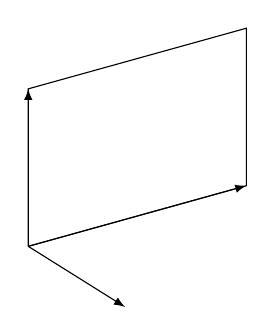
\begin{tikzpicture}
		\draw (-1,-1,1) -- (-1,1,1) -- (1,1,-1) -- (1,-1,-1) -- (-1,-1,1);
		\draw[-latex] (-1,-1,1) -- (-1,1,1);		
		\draw[-latex] (-1,-1,1) -- (1,-1,-1);		
		\draw[-latex] (-1,-1,1) -- (1,-1,3);
	\end{tikzpicture}
\end{figure}

\begin{align*}
&&p_i\overset{\text{World}}{=}&R_\text{Tex}\cdot\vektor{u_i\\v_i\\0}&&\\
&&&\overset{\rotatebox{90}{$=$}}{[t,b,n]}
\end{align*}
\begin{align*}
&&p_i-p_j &=R\cdot\vektor{u_i-u_j\\v_i-v_j\\0}&&\\
&&[p_1-p_2,p_2-p_3,p_3-p_1] &=R\cdot\vektor{u_1-u_2&u_2-u_3&u_3-u_1\\v_1-v_2&v_2-v_3&v_3-v_1\\0&0&0}
\end{align*}
\begin{tikzpicture}
\node (A) {
	$
	\vektor{(p_1-p_2)^T\\(p_2-p_3)^T\\(p_3-p_1)^T} = \vektor{u_1-u_2&v_1-v_2&0\\u_2-u_3&v_2-v_3&0\\u_3-u_1&v_3-v_1&0\\}\cdot\vektor{t^T\\b^T\\n^T}
	$
	};
	\draw ($(A.south east)+(0,.35)$) -- ($(A.south west)+(0,.35)$);
\end{tikzpicture}